\chapter{Introduction}
Classical lasers, such as a laser pointer or a Helium-Neon gas laser, are limited to a single wavelength since the light is generated by stimulated emission. Tuneable lasers on the other hand, have the ability to operate within a range of wavelengths \cite{bohun, burgoyne2010, yamashita}. As a result, tuneable lasers have applications in spectroscopy and high resolution imaging such as coherent anti-Stokes Raman spectroscopy and optical coherence tomography \cite{bohun, burgoyne2014, yamashita}. This article is concerned with dispersion-tuned actively mode-locked (DTAML) lasers. The laser cavity consists of four elements: the dispersive element, the modulator, the gain fibre, and the optical coupler. The gain fibre consists of either an Erbium or Ytterbium doped fibre, and dispersion is generated by the highly dispersive chirped fibre Bragg grating (CFBG). \\

To start off the discussion of the current modelling efforts for a tuneable laser, we begin with a review of the efforts to describe an `average' model. The idea is to capture some of the physical elements in the waveform described by an effective PDE, the solution of which gives the amplitude of the wave packet.

\begin{figure}[htbp]
\centering
% !TeX root = ../Thesis.tex

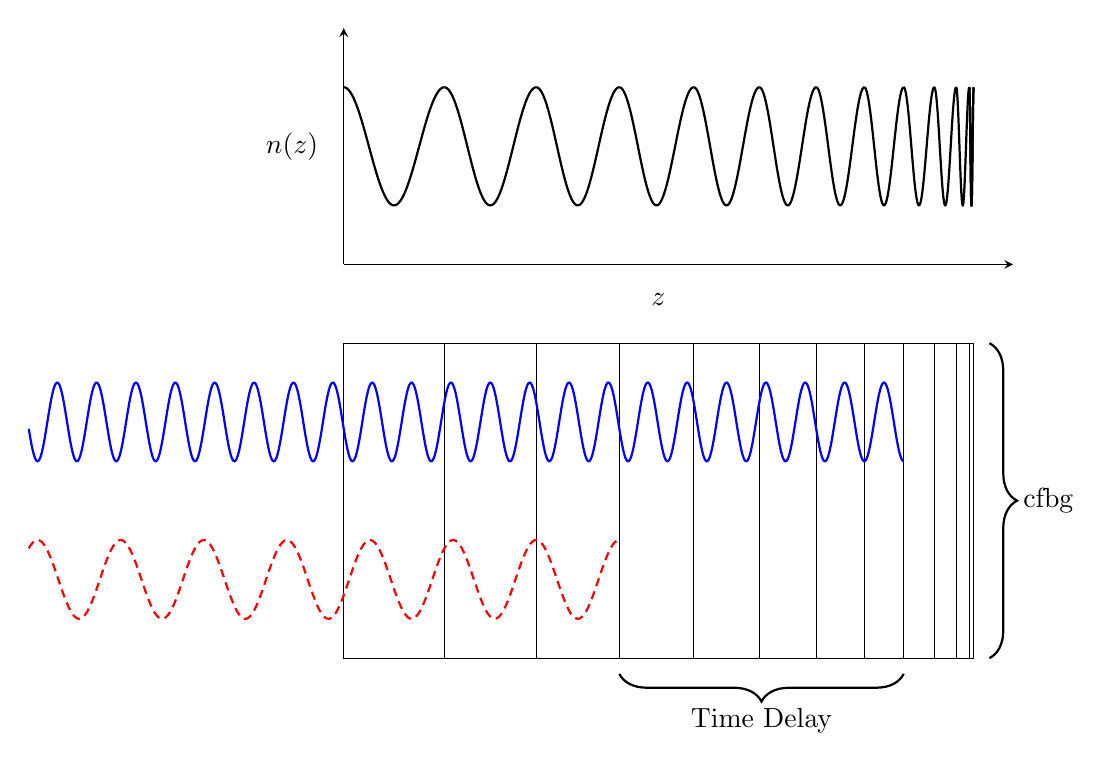
\begin{tikzpicture}
% CFBG
\draw (4,0) -- (12,0) -- (12,4) -- (4,4) -- cycle;
\foreach \i in {1,...,12}
  \draw (12 - 1/18*\i*\i,0) -- (12 - 1/18*\i*\i,4);
%\foreach \i in {0,...,12}
%  \draw [dashed] (12 - 1/18*\i*\i,4) -- (12 - 1/18*\i*\i,8);
% Waves
\draw [domain=0:(12-16/18), samples=1000, blue, thick] plot (\x, {-0.5*cos(4*pi*(\x-(12-25/18)) r) + 3});
\draw [domain=0:(12-81/18), samples=500, red, thick, densely dashed] plot (\x, {0.5*cos(2*pi*36/38*(\x-(12-100/18)) r) + 1});

% Labels
\draw [thick, decorate, decoration={brace, mirror, raise=0.2cm, amplitude=10pt}] (7.5,0) -- (100/9,0)
node [pos=0.5,anchor=north,yshift=-0.5cm] {Time Delay};
\draw [thick, decorate, decoration={brace, mirror, raise=0.2cm, amplitude=10pt}] (12,0) -- (12,4)
node [pos=0.5,anchor=west,xshift=0.5cm] {\gls{cfbg}};

% Index of refraction
\draw [->, >=stealth] (4,5) -- (12.5,5)
node [pos=0.47,anchor=north,yshift=-0.25cm] {$z$};
\draw [->, >=stealth] (4,5) -- (4,8)
node [pos=0.5,anchor=east,xshift=-0.2cm] {$n(z)$};
\foreach \i in {0,...,12}
  \draw [domain=(12-\i*\i/18):(12-(\i-1)*(\i-1)/18), samples=100, black, thick] plot (\x, {3/4*cos(2*pi*36/(4*\i-2)*(\x-(12-\i*\i/18)) r) + 6.5});
\end{tikzpicture}
\label{fig:cfbg}
\caption[Chirped Fibre Bragg Grating]{Chirped fibre Bragg grating schematic.}
\end{figure}